\section{Περιβάλλον ανάπτυξης και εργαλεία}
Η εφαρμογή αναπτύχθηκε με Spring Boot και React, ενώ για τη σχεσιακή
αποθήκευση χρησιμοποιείται MySQL. Η συσκευασία και η εκτέλεση των επιμέρους
υπηρεσιών βασίζονται σε Docker και Docker Compose. Για τη διαχείριση αρχείων
και την ασφαλή απομακρυσμένη πρόσβαση χρησιμοποιούνται SSH/SFTP και
Cyberduck, ενώ η διαχείριση των πόρων νέφους πραγματοποιείται από την κονσόλα
AWS.
\section{Δημιουργία και διαχείριση εικόνων Docker}
Η εγκατάσταση περιλαμβάνει τρία containers: \texttt{petclinic-mysql} με
MySQL~8.4, \texttt{petclinic-app} με την εφαρμογή Spring Boot και
\texttt{petclinic-nginx} με Nginx~1.27 Alpine. Οι υπηρεσίες φέρουν πολιτική
\texttt{restart: unless-stopped}. Η υπηρεσία Docker ρυθμίστηκε να εκκινεί
μαζί με το λειτουργικό σύστημα. Έτσι, μετά από reboot του EC2 instance, η
πολιτική επανεκκίνησης ενεργοποιεί αυτόματα και τα τρία containers.

\begin{figure}[htbp]
\centering
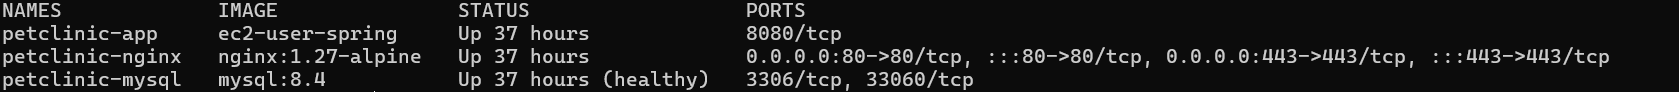
\includegraphics[width=\textwidth]{figures/infrastructure/docker-running-containers.png}
\caption{Κατάσταση των containers της παραγωγικής εγκατάστασης. Η εφαρμογή,
ο Nginx και η MySQL εκτελούνται ταυτόχρονα, ενώ η MySQL αναφέρεται ως
\texttt{healthy}.}
\label{fig:docker-running-containers}
\end{figure}
\section{Παραμετροποίηση της εφαρμογής ανά περιβάλλον}
Τα στοιχεία σύνδεσης της βάσης δεδομένων, το JWT signing secret, το bootstrap
password και τα credentials εξωτερικών υπηρεσιών παρέχονται μέσω environment
variables. Το πραγματικό αρχείο \texttt{.env} δεν συμπεριλαμβάνεται στο
version control, ενώ στο repository διατηρείται μόνο αρχείο παραδείγματος με
τα ονόματα των απαιτούμενων μεταβλητών. Με τον τρόπο αυτό το ίδιο application
package μπορεί να χρησιμοποιείται σε local και production περιβάλλον χωρίς
ενσωμάτωση μυστικών στον πηγαίο κώδικα.

\section{Ενσωμάτωση Google Calendar και Amazon SES}
Η εφαρμογή υποστηρίζει σύνδεση λογαριασμού Google Calendar μέσω OAuth~2.0.
Μετά από ρητή εξουσιοδότηση του χρήστη, τα ραντεβού μπορούν να
αντιστοιχίζονται με calendar events. Το OAuth client identifier και το client
secret δεν αποθηκεύονται στον κώδικα, αλλά παρέχονται κατά το deployment μέσω
environment variables, μαζί με το εγκεκριμένο callback URL του production
domain. Για την ελεγχόμενη δοκιμή δημιουργήθηκε ανεξάρτητο Google Cloud
project, ενεργοποιήθηκε το Google Calendar API και διαμορφώθηκε εφαρμογή
OAuth τύπου External σε κατάσταση Testing. Ο λογαριασμός του έργου ορίστηκε
ως ο μοναδικός test user και ο Web OAuth client δέχεται ως redirect URI το
\path{https://thesis-tasiopoulos.com/auth/google/callback}. Τα νέα
credentials αποθηκεύτηκαν εκτός repository και δεν εμφανίζονται στα τεκμήρια.
Στο production περιβάλλον μεταφέρθηκαν μέσω κρυφής εισόδου τερματικού στο
προστατευμένο αρχείο \texttt{.env} και αντιστοιχίστηκαν αποκλειστικά στο Spring
container μέσω Docker Compose. Μετά την επαναδημιουργία μόνο του Spring
container επαληθεύτηκαν η παρουσία των τριών μεταβλητών, η επιτυχής εκκίνηση
της εφαρμογής και απόκριση HTTP~200 από το δημόσιο HTTPS endpoint.

Η λειτουργία εκτίθεται από τη σελίδα \enquote{Profile \& Integrations}, στην
οποία ο χρήστης μεταβαίνει και από την κάρτα ονόματος και avatar της
πλευρικής πλοήγησης. Η σελίδα διαχωρίζει σκόπιμα δύο έννοιες: το email
επικοινωνίας του λογαριασμού Happy Tails και το email του εξουσιοδοτημένου
Google Calendar. Το πρώτο εξακολουθεί να υπόκειται στον μοναδικό περιορισμό
της βάσης δεδομένων, ενώ το δεύτερο αποθηκεύεται στο ξεχωριστό πεδίο
\texttt{calendarEmail}. Επομένως ένας ήδη χρησιμοποιούμενος Google λογαριασμός
μπορεί να συνδεθεί ως πάροχος ημερολογίου χωρίς να μετονομάσει τον χρήστη ή να
συγκρουστεί με το email άλλου application account, όπως του administrator.

Με την επιλογή \enquote{Connect Google Calendar} το backend δημιουργεί τυχαία
τιμή \texttt{state}, τη συνδέει με τον ενεργό χρήστη σε βραχύβιο server-side
session και ανακατευθύνει στη σελίδα συγκατάθεσης της Google. Ζητούνται τα
scopes Calendar, OpenID, email και profile. Στην επιστροφή, το callback
ελέγχει κωδικό και \texttt{state} πριν ανταλλάξει τον authorization code με
access και refresh token. Τα tokens δεν επιστρέφονται στο React frontend και
δεν εμφανίζονται στα στιγμιότυπα. Η διαδρομή αποτελέσματος OAuth επιτρέπεται
να φορτωθεί δημόσια ώστε να εμφανίσει το αποτέλεσμα της εξωτερικής
ανακατεύθυνσης, ενώ η επόμενη μετάβαση στο profile προστατεύεται κανονικά από
το JWT cookie. Το session cookie έχει \texttt{HttpOnly}, \texttt{Secure} και
\texttt{SameSite=Lax}, ώστε να διατηρείται ο έλεγχος \texttt{state} κατά την
επιστροφή από τη Google χωρίς να γίνεται προσβάσιμο από JavaScript.

Μετά τη σύνδεση, η δημιουργία ραντεβού επιχειρεί εισαγωγή event, η αλλαγή
ημερομηνίας ή στοιχείων εκτελεί patch και η διαγραφή ραντεβού διαγράφει το
αντίστοιχο event. Το αναγνωριστικό του Google event αποθηκεύεται στο
ραντεβού, ώστε η εφαρμογή να γνωρίζει αν απαιτείται δημιουργία ή ενημέρωση.
Επειδή τα ραντεβού αποθηκεύονται ως τοπικές τιμές χωρίς offset, η μετατροπή
προς και από Google Calendar χρησιμοποιεί ρητά την IANA ζώνη
\texttt{Europe/Athens}, μαζί με τους κανόνες θερινής ώρας, και όχι την
προεπιλεγμένη ζώνη UTC του container. Η Google χρησιμοποιεί την ίδια χρονική
πληροφορία για την εμφάνιση του event και για τις προσκλήσεις που αποστέλλει
στους attendees· η εφαρμογή δεν δημιουργεί δεύτερο αρχείο iCalendar μέσω SES.

Η τελική δοκιμή επιβεβαίωσε ότι το ίδιο ραντεβού εμφανίζεται στις 09:30 τόσο
στην εφαρμογή (Σχήμα~\ref{fig:calendar-app-time}) όσο και στο Google Calendar,
ενώ η πρόσκληση αναγράφει επίσης 09:30--10:00 και τη ζώνη Eastern European
Time--Athens (Σχήμα~\ref{fig:calendar-google-evidence}).

\begin{figure}[htbp]
\centering
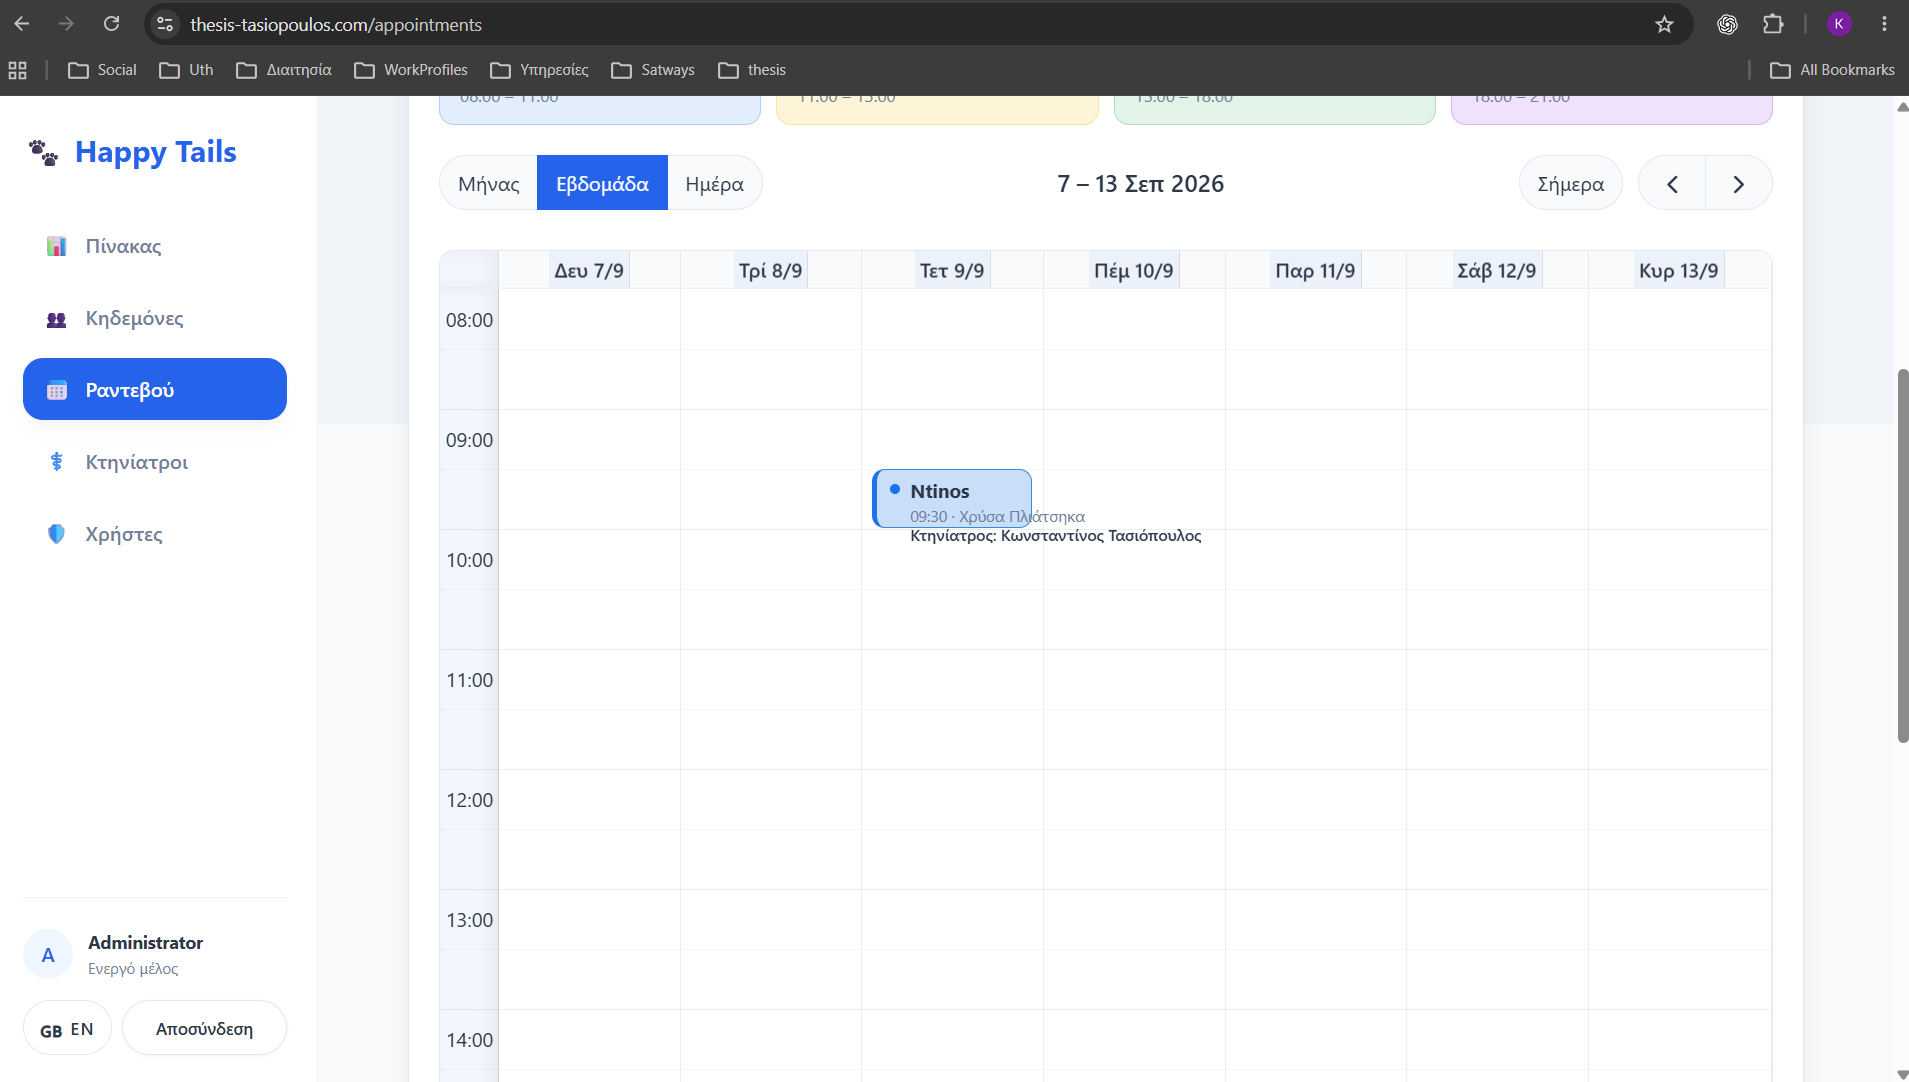
\includegraphics[width=0.96\textwidth]{figures/application/google-calendar-app-0930.png}
\caption{Το δοκιμαστικό ραντεβού στις 09:30 στην εβδομαδιαία προβολή του
Happy Tails μετά τη διόρθωση της ζώνης ώρας.}
\label{fig:calendar-app-time}
\end{figure}

\begin{figure}[htbp]
\centering
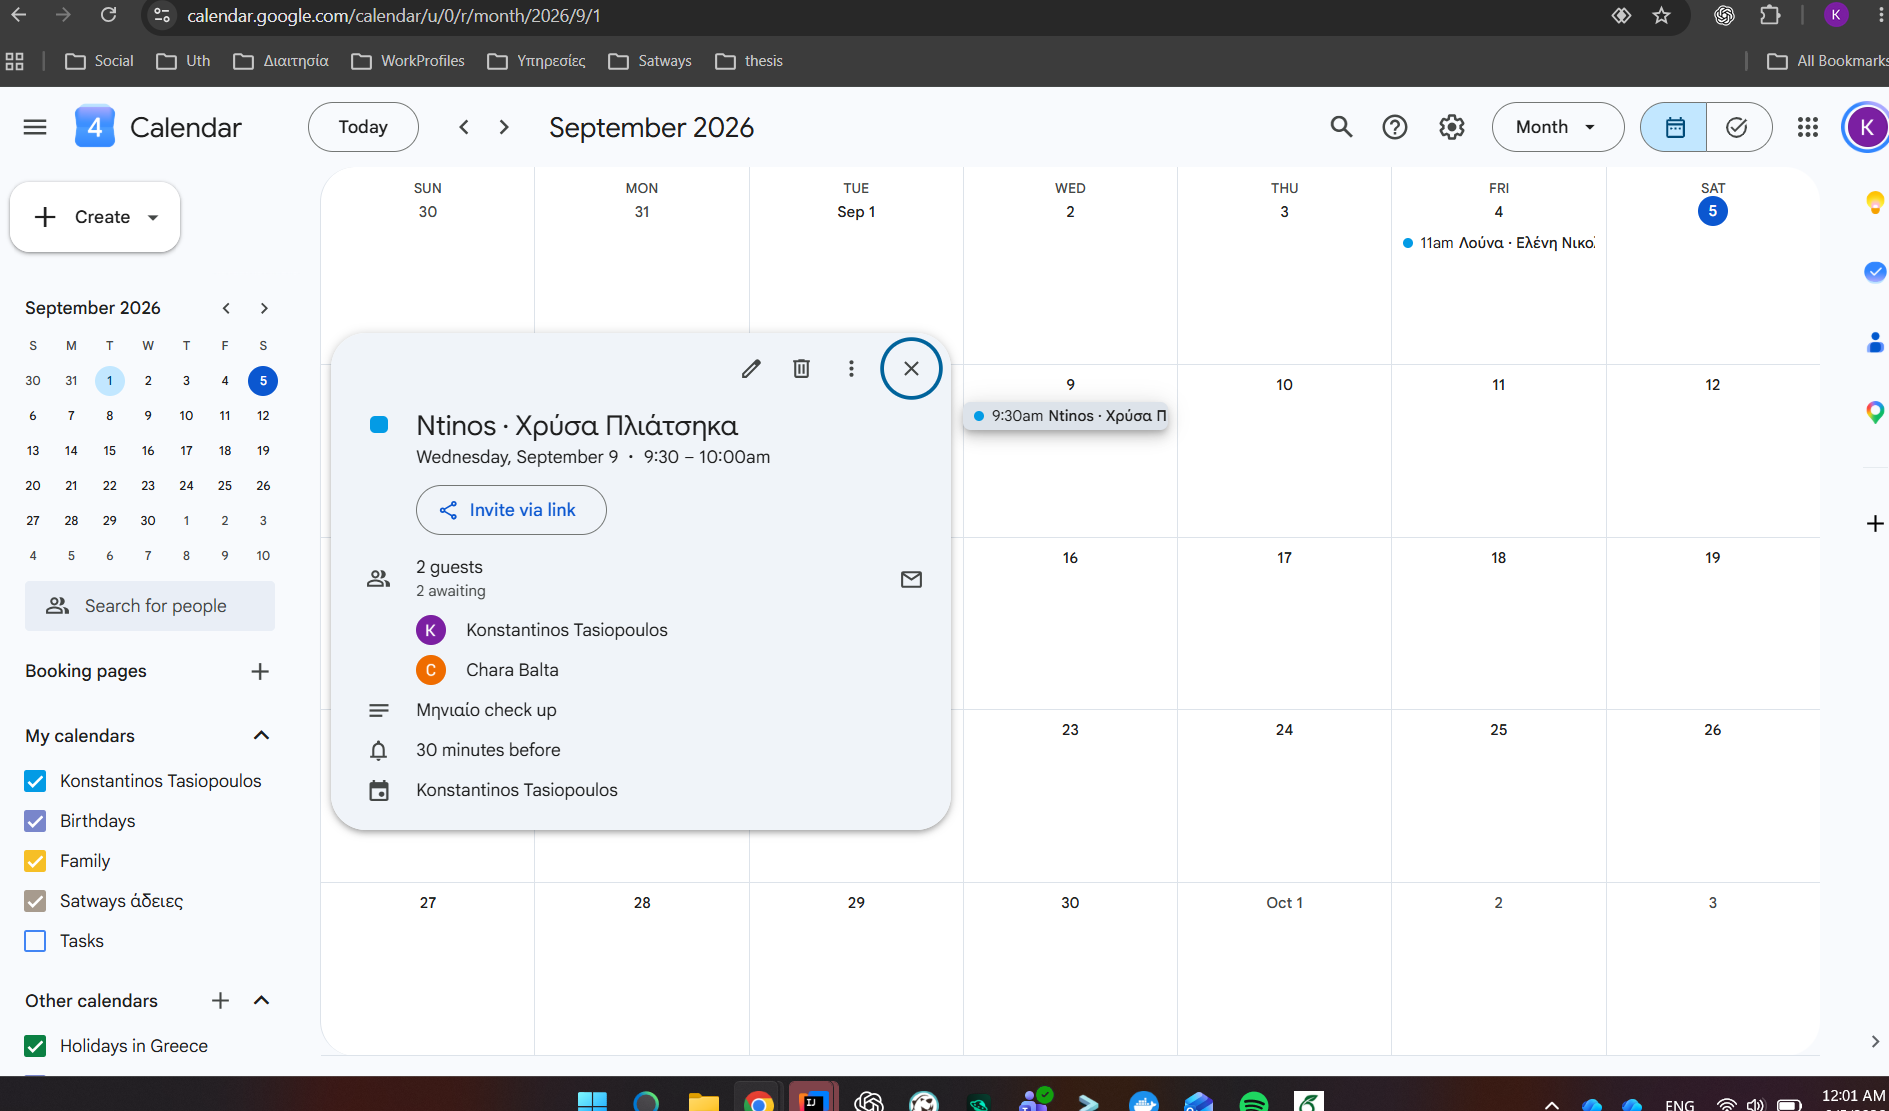
\includegraphics[width=0.78\textwidth]{figures/application/google-calendar-event-0930.png}\par\medskip
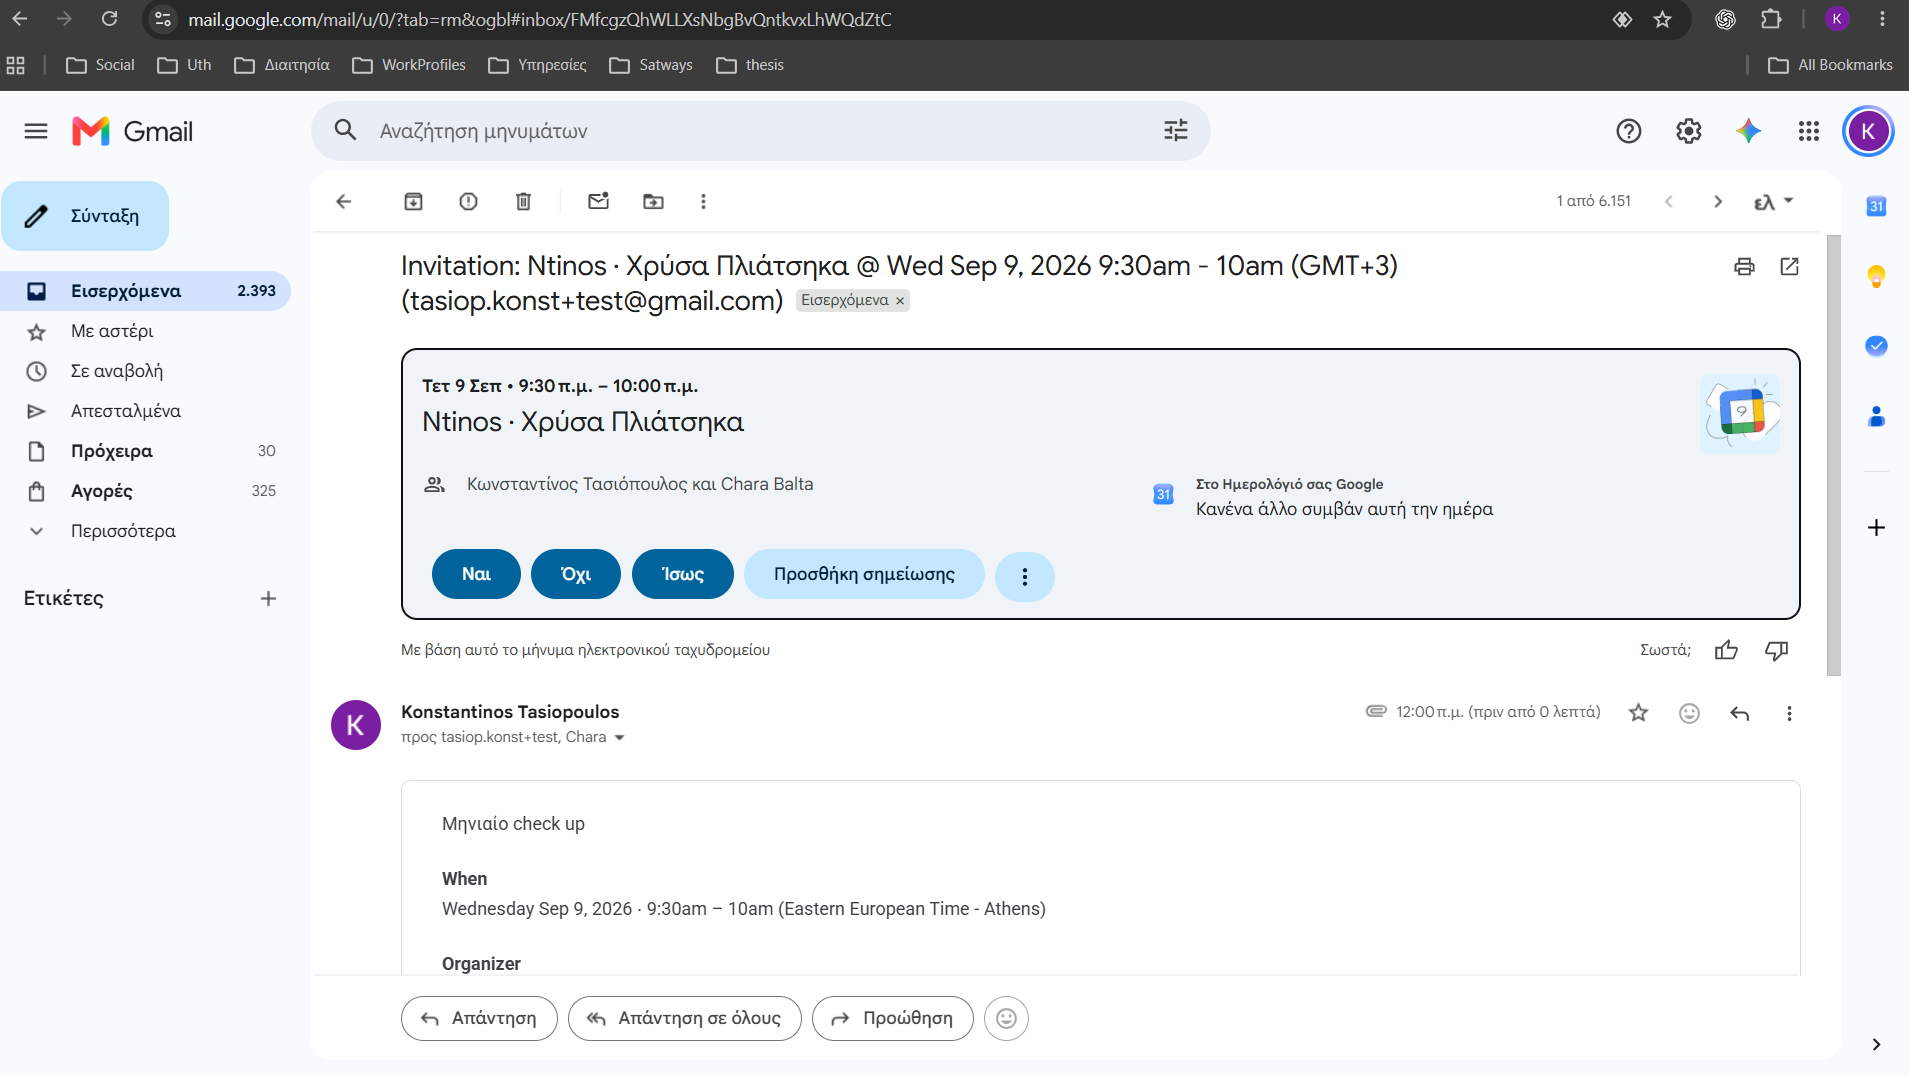
\includegraphics[width=0.78\textwidth]{figures/application/google-calendar-invitation-email.png}
\caption{Το ίδιο event στο Google Calendar και η αντίστοιχη πρόσκληση email,
με συμφωνία ώρας 09:30 και διάρκεια τριάντα λεπτών. Ο administrator/organizer
και η client owner αποτελούν διαφορετικούς δοκιμαστικούς παραλήπτες.}
\label{fig:calendar-google-evidence}
\end{figure}

Το Amazon SES και το Google Calendar αποτελούν δύο ανεξάρτητες εξωτερικές
ενσωματώσεις και δεν επικοινωνούν απευθείας μεταξύ τους. Το Happy Tails είναι
το κοινό σημείο ενορχήστρωσης, αλλά τους αναθέτει διαφορετικές ευθύνες. Η
υπηρεσία Calendar καλεί το Google Calendar API με OAuth tokens για create,
patch ή delete του event και χρησιμοποιεί \texttt{sendUpdates=all}, οπότε η
ίδια η Google αποστέλλει προσκλήσεις, ενημερώσεις και ακυρώσεις στους
attendees. Το Amazon SES δεν συμμετέχει στη ροή ραντεβού· χρησιμοποιείται
αποκλειστικά για verification και password reset των λογαριασμών προσωπικού
της εφαρμογής.

Ο Πίνακας~\ref{tab:external-notification-triggers} αποσαφηνίζει πότε
ενεργοποιείται κάθε μηχανισμός. Ο διαχωρισμός αποτρέπει διπλές ειδοποιήσεις
και δεν υποχρεώνει τους πελάτες να διαθέτουν λογαριασμό Happy Tails ή verified
SES identity.

\begin{table}[htbp]
\centering
\caption{Διάκριση trigger, καναλιού και παραληπτών για Google Calendar και
Amazon SES.}
\label{tab:external-notification-triggers}
\small
\begin{tabularx}{\textwidth}{p{0.19\textwidth} X X}
\toprule
\textbf{Trigger} & \textbf{Google Calendar} & \textbf{Amazon SES} \\
\midrule
Νέος λογαριασμός & Δεν ενεργοποιείται. & Στέλνει verification link διάρκειας
24 ωρών στο email του νέου application user. \\
Αίτημα επαναφοράς κωδικού & Δεν ενεργοποιείται. & Στέλνει link διάρκειας
60 λεπτών στο email υπάρχοντος, επιβεβαιωμένου application user. \\
Δημιουργία ραντεβού & Εισάγει event και η Google ειδοποιεί τους attendees. &
Δεν ενεργοποιείται. \\
Ενημέρωση ή μεταφορά & Εκτελεί patch του event και ενημερώνει attendees. &
Δεν ενεργοποιείται. \\
Διαγραφή ραντεβού & Διαγράφει το event και η Google στέλνει cancellation. &
Δεν ενεργοποιείται. \\
Διοικητική έγκριση λογαριασμού & Δεν ενεργοποιείται. & Δεν αποστέλλεται
ξεχωριστό μήνυμα στον administrator ή στον αιτούντα στην παρούσα έκδοση. \\
\bottomrule
\end{tabularx}
\end{table}

Ο όρος client owner δηλώνει τον κηδεμόνα ζώου, ο οποίος αποθηκεύεται ως
εγγραφή \texttt{Owner} και δεν συνδέεται στην εσωτερική εφαρμογή. Αντίθετα, ο
ρόλος \texttt{CLINIC\_OWNER} ανήκει σε \texttt{AppUser} του προσωπικού. Οι
κηδεμόνες λαμβάνουν Calendar notifications στη διεύθυνση της εγγραφής τους
χωρίς OAuth σύνδεση ή SES verification. Τα verification και password-reset
μηνύματα του SES απευθύνονται μόνο στον \texttt{AppUser} προσωπικού που
εκτελεί την αντίστοιχη ροή. Ο administrator δεν λαμβάνει αυτοματοποιημένο SES
email για νέα εκκρεμή εγγραφή· ενημερώνεται από τη λίστα
\enquote{Εκκρεμείς εγκρίσεις} και πραγματοποιεί την ξεχωριστή διοικητική
έγκριση μέσα στην εφαρμογή.

Επειδή η πειραματική εγκατάσταση λειτουργεί σε SES sandbox, κάθε διεύθυνση
προσωπικού στην οποία επιχειρεί να παραδώσει το SES πρέπει πρώτα να έχει
επιβεβαιωθεί ως SES identity. Πρόκειται για υποδομικό προαπαιτούμενο και όχι
για έγκριση χρήστη: (1) το SES επιτρέπει την παράδοση στον verified
δοκιμαστικό παραλήπτη, (2) ο χρήστης επιβεβαιώνει μέσω του συνδέσμου ότι
ελέγχει το email του και (3) ο administrator εγκρίνει την πρόσβαση στην
εφαρμογή. Η απαίτηση (1) παύει για γενικούς παραλήπτες μετά την έγκριση
production access από την AWS, ενώ οι έλεγχοι (2) και (3) παραμένουν
λειτουργίες του Happy Tails. Η διεύθυνση του client owner δεν χρειάζεται SES
verification, επειδή χρησιμοποιείται μόνο ως attendee του Google event.

Στο ελεγχόμενο σενάριο επίδειξης ο administrator/organizer και η client
owner/attendee χρησιμοποιούν διαφορετικές διευθύνσεις και ανεξάρτητες
θυρίδες email. Τυχόν βασική διεύθυνση Gmail και plus alias που σχετίζονται
με τον λογαριασμό του administrator παραμένουν παραλλαγές της δικής του
θυρίδας και δεν αποτελούν τη διεύθυνση της client owner. Έτσι η δοκιμή
καλύπτει πραγματική παράδοση της πρόσκλησης σε διακριτό παραλήπτη ιδιοκτήτη.

Αν η εξωτερική υπηρεσία αποτύχει, η βασική συναλλαγή της κλινικής δεν
αναιρείται: το ραντεβού παραμένει στη MySQL και εμφανίζεται ως εκκρεμές για
αυτόματη επανάληψη όταν ανακτηθεί ξανά η εβδομαδιαία προβολή. Η τελική
end-to-end επαλήθευση ολοκληρώνεται με σύνδεση του δοκιμαστικού λογαριασμού
και καταγραφή της δημιουργίας, ενημέρωσης και ακύρωσης ενός event.

Για τη ροή εγγραφής υλοποιήθηκε ξεχωριστή επιβεβαίωση διεύθυνσης email. Η
εφαρμογή παράγει τυχαίο token 256~bit με \texttt{SecureRandom}, αποθηκεύει στη
MySQL μόνο το SHA-256 hash του και αποστέλλει σύνδεσμο χρονικής ισχύος 24
ωρών. Έτσι, ακόμη και αν διαβαστεί ο πίνακας των tokens, η τιμή που απαιτείται
για την επιβεβαίωση δεν είναι άμεσα διαθέσιμη. Με την πρώτη επιτυχή χρήση το
token διαγράφεται. Η επιβεβαίωση email και η έγκριση από administrator
παραμένουν δύο διακριτά βήματα: το πρώτο αποδεικνύει ότι ο χρήστης ελέγχει τη
διεύθυνση, ενώ το δεύτερο επιτρέπει στην κλινική να αποφασίσει αν ο νέος
λογαριασμός θα αποκτήσει πρόσβαση στο εσωτερικό σύστημα.

Η αποστολή πραγματοποιείται από το Spring Boot \texttt{JavaMailSender} προς
το SMTP endpoint του Amazon SES στην περιοχή Frankfurt
\cite{rfc5321,aws2026sessmtp}. Οι παράμετροι host,
port, username, password, STARTTLS, sender address και public base URL
περνούν στο application container ως environment variables του Docker
Compose. Το application package επομένως δεν περιέχει SMTP credentials και
η ίδια έκδοση μπορεί να λειτουργήσει με διαφορετικές ρυθμίσεις στο local και
στο production περιβάλλον. Η AWS πλευρά της διαμόρφωσης και η ανεξάρτητη
δοκιμαστική αποστολή παρουσιάστηκαν στην
Εικόνα~\ref{fig:amazon-ses-evidence}.

Η λειτουργική δοκιμή εκτελέστηκε με νέο λογαριασμό και verified παραλήπτη του
SES sandbox. Η φόρμα εγγραφής επέστρεψε επιτυχές αποτέλεσμα, το μήνυμα
παραδόθηκε στο mailbox και ο σύνδεσμος μετέφερε τον χρήστη στη σελίδα
επιτυχούς επιβεβαίωσης. Η προσπάθεια σύνδεσης πριν από την έγκριση απορρίφθηκε
ως αναμενόταν. Στη συνέχεια ο administrator εντόπισε την αίτηση, ενεργοποίησε
τον λογαριασμό, απέδωσε τον ρόλο ιδιοκτήτη κλινικής και η σύνδεση ολοκληρώθηκε
με πρόσβαση στον πίνακα ελέγχου. Τα τέσσερα σημεία ελέγχου φαίνονται στην
Εικόνα~\ref{fig:registration-email-approval-flow}.

Για την ελεγχόμενη επαναχρησιμοποίηση των περιορισμένων δοκιμαστικών
διευθύνσεων προστέθηκε στη διαχείριση χρηστών δυνατότητα διαγραφής λογαριασμού
προσωπικού. Η ενέργεια εκτελείται μόνο από administrator, ζητά επιβεβαίωση
στον browser και δεν διατίθεται για λογαριασμό με ρόλο
\texttt{SUPERADMIN}. Επιτρέπεται για απλό προσωπικό, ιδιοκτήτη κλινικής ή
κτηνίατρο μόνο όταν ο λογαριασμός δεν συνδέεται με ιστορικό ραντεβού· σε
αντίθετη περίπτωση το backend επιστρέφει HTTP~409 και ο λογαριασμός πρέπει να
απενεργοποιηθεί αντί να διαγραφεί. Μετά τη διαγραφή ενός μη χρησιμοποιούμενου
λογαριασμού, το username και το email μπορούν να χρησιμοποιηθούν σε νέα
εγγραφή, η οποία ενεργοποιεί από την αρχή την κανονική ροή επιβεβαίωσης μέσω
Amazon SES και διοικητικής έγκρισης.

\begin{figure}[htbp]
\centering
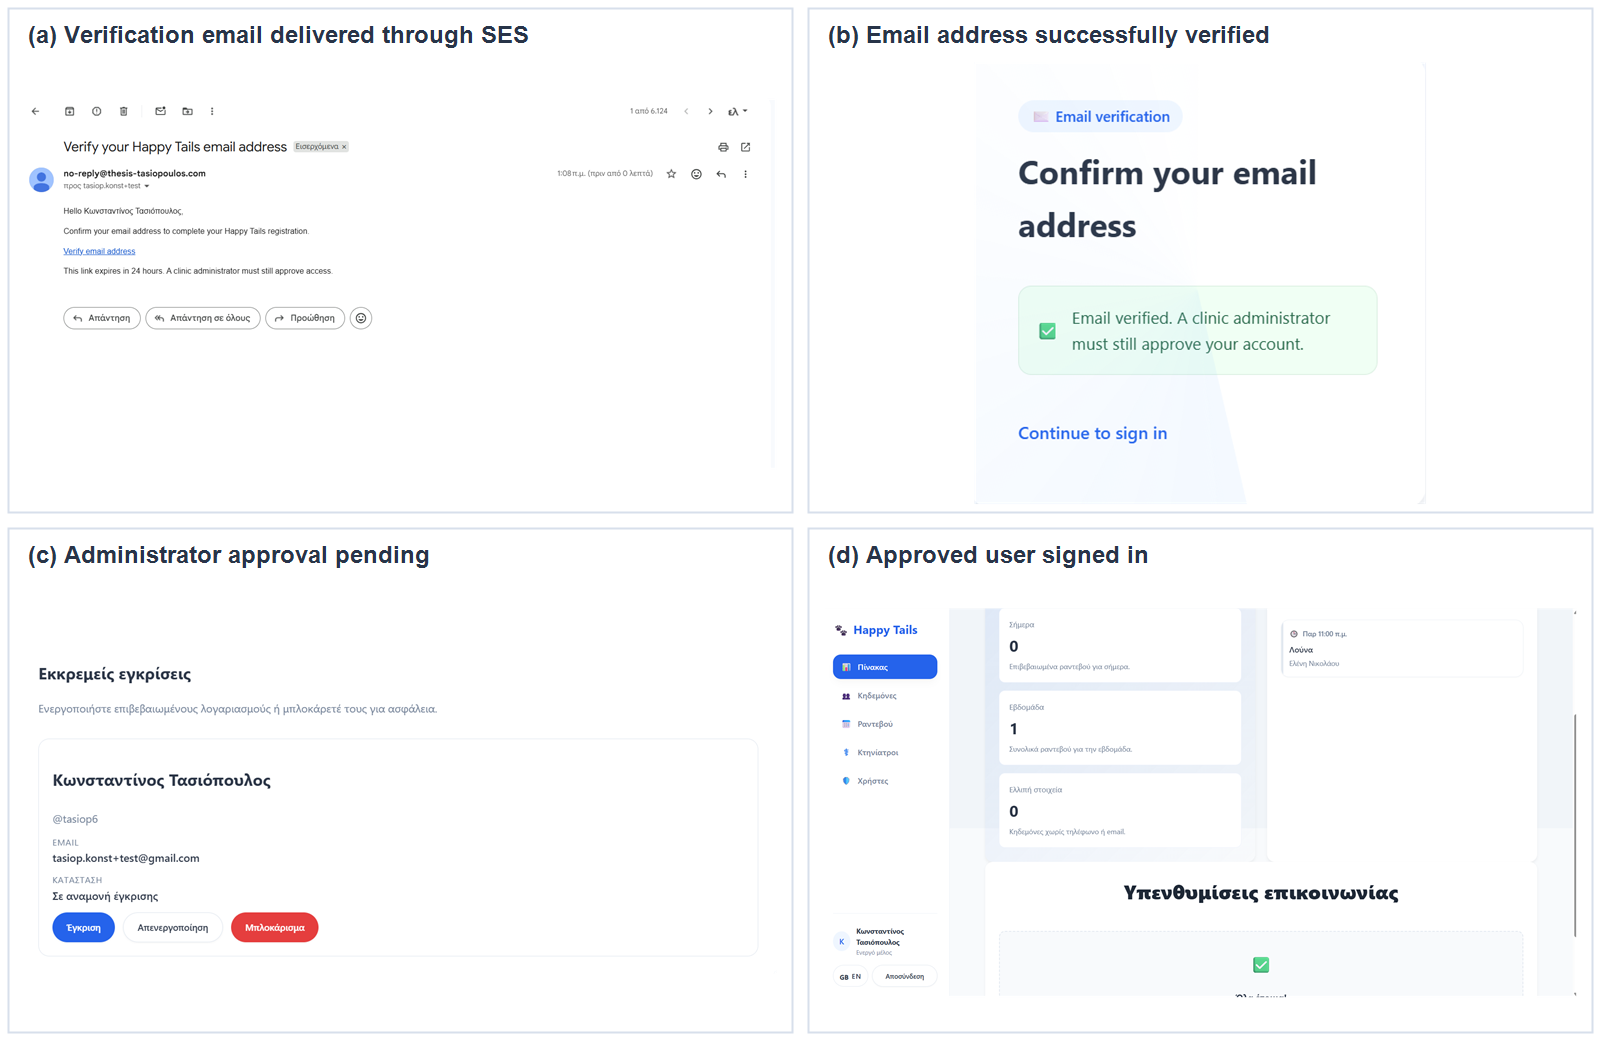
\includegraphics[width=\textwidth]{figures/application/registration-email-approval-flow.png}
\caption{End-to-end ροή νέου λογαριασμού: παράδοση verification email μέσω
SES, επιβεβαίωση διεύθυνσης, εκκρεμής έγκριση από administrator και επιτυχής
είσοδος του ενεργοποιημένου χρήστη.}
\label{fig:registration-email-approval-flow}
\end{figure}

Η ίδια υποδομή email αξιοποιήθηκε και για την ασφαλή επαναφορά κωδικού. Η
σελίδα εισόδου οδηγεί σε φόρμα όπου ζητείται μόνο η διεύθυνση email. Η
απόκριση παραμένει ίδια είτε υπάρχει ο λογαριασμός είτε όχι, ώστε να μην
αποκαλύπτεται σε τρίτους ποια email είναι καταχωρισμένα. Για υπαρκτό και
επαληθευμένο λογαριασμό δημιουργείται νέο τυχαίο token, αποθηκεύεται μόνο το
hash του και αποστέλλεται σύνδεσμος ισχύος 60 λεπτών. Η νέα τιμή του κωδικού
αποθηκεύεται με τον \texttt{PasswordEncoder} του Spring Security και το token
καταναλώνεται αμέσως, ώστε ο ίδιος σύνδεσμος να μην μπορεί να χρησιμοποιηθεί
δεύτερη φορά. Η υλοποίηση ελέγχθηκε με tests για έγκυρο, ληγμένο και κενό
token και στη συνέχεια με πραγματική αποστολή μέσω SES. Η
Εικόνα~\ref{fig:password-reset-flow} παρουσιάζει τα βασικά στάδια χωρίς να
εμφανίζει την τιμή του token.

\begin{figure}[htbp]
\centering
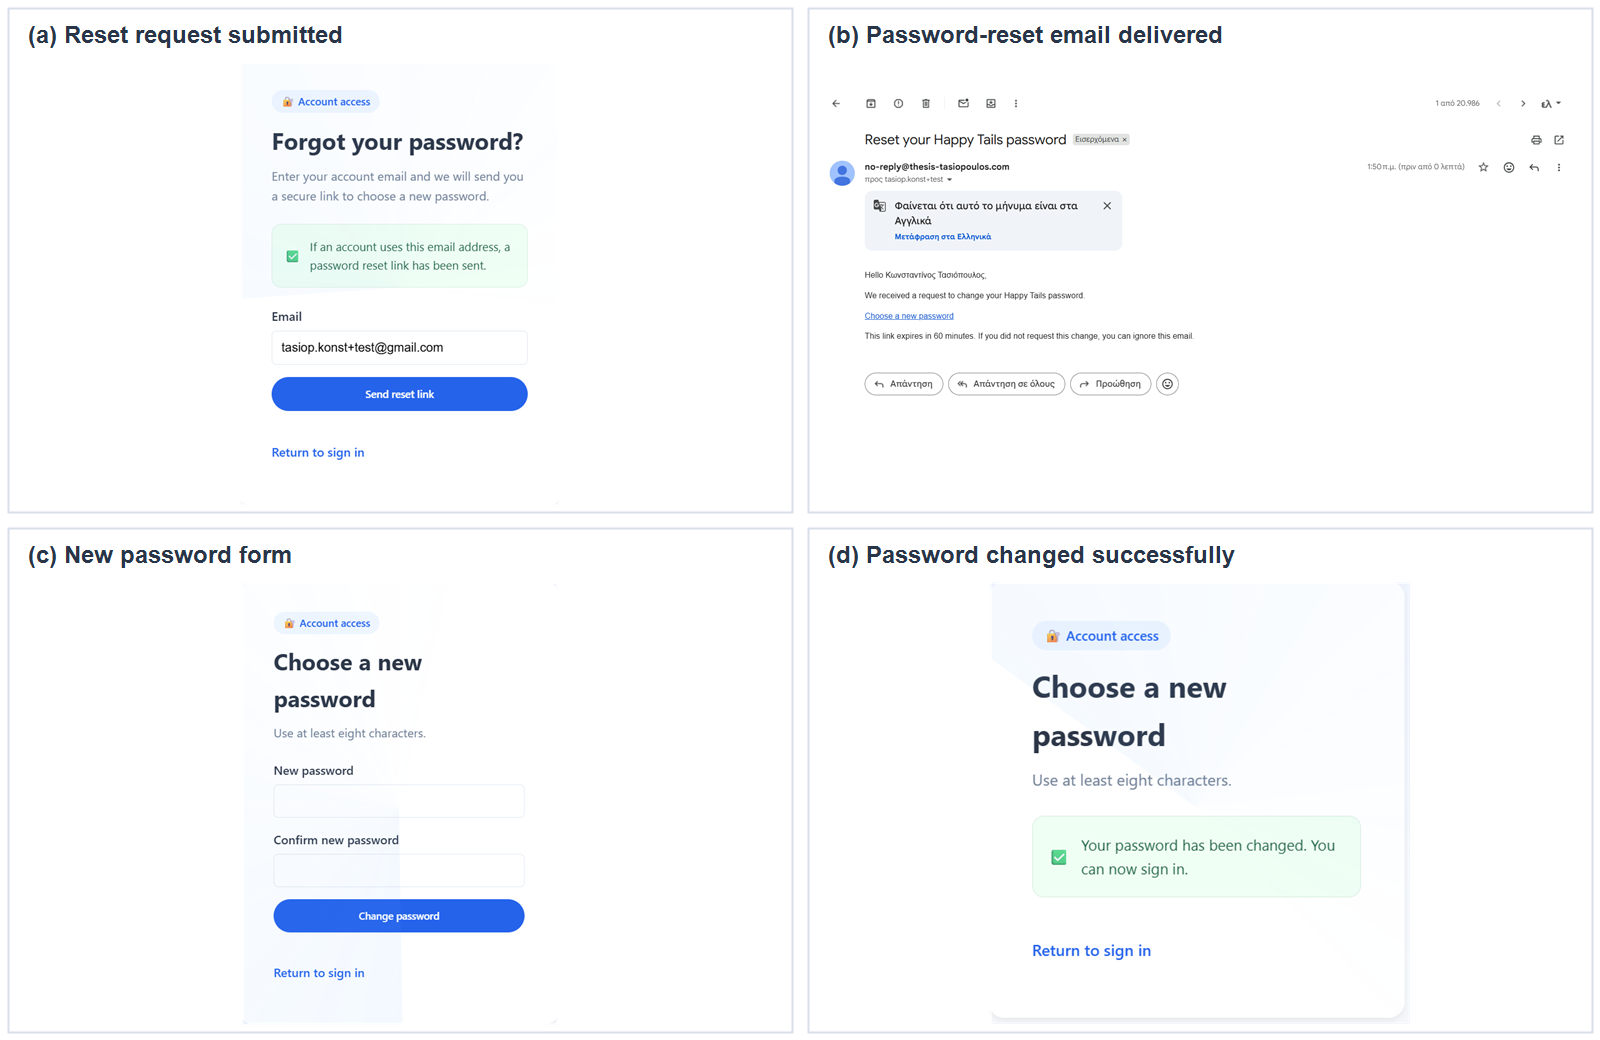
\includegraphics[width=\textwidth]{figures/application/password-reset-flow.png}
\caption{Ροή επαναφοράς κωδικού: ουδέτερη επιβεβαίωση του αιτήματος,
παράδοση email μέσω SES, εισαγωγή νέου κωδικού και επιτυχής ολοκλήρωση.}
\label{fig:password-reset-flow}
\end{figure}

\begin{figure}[htbp]
\centering
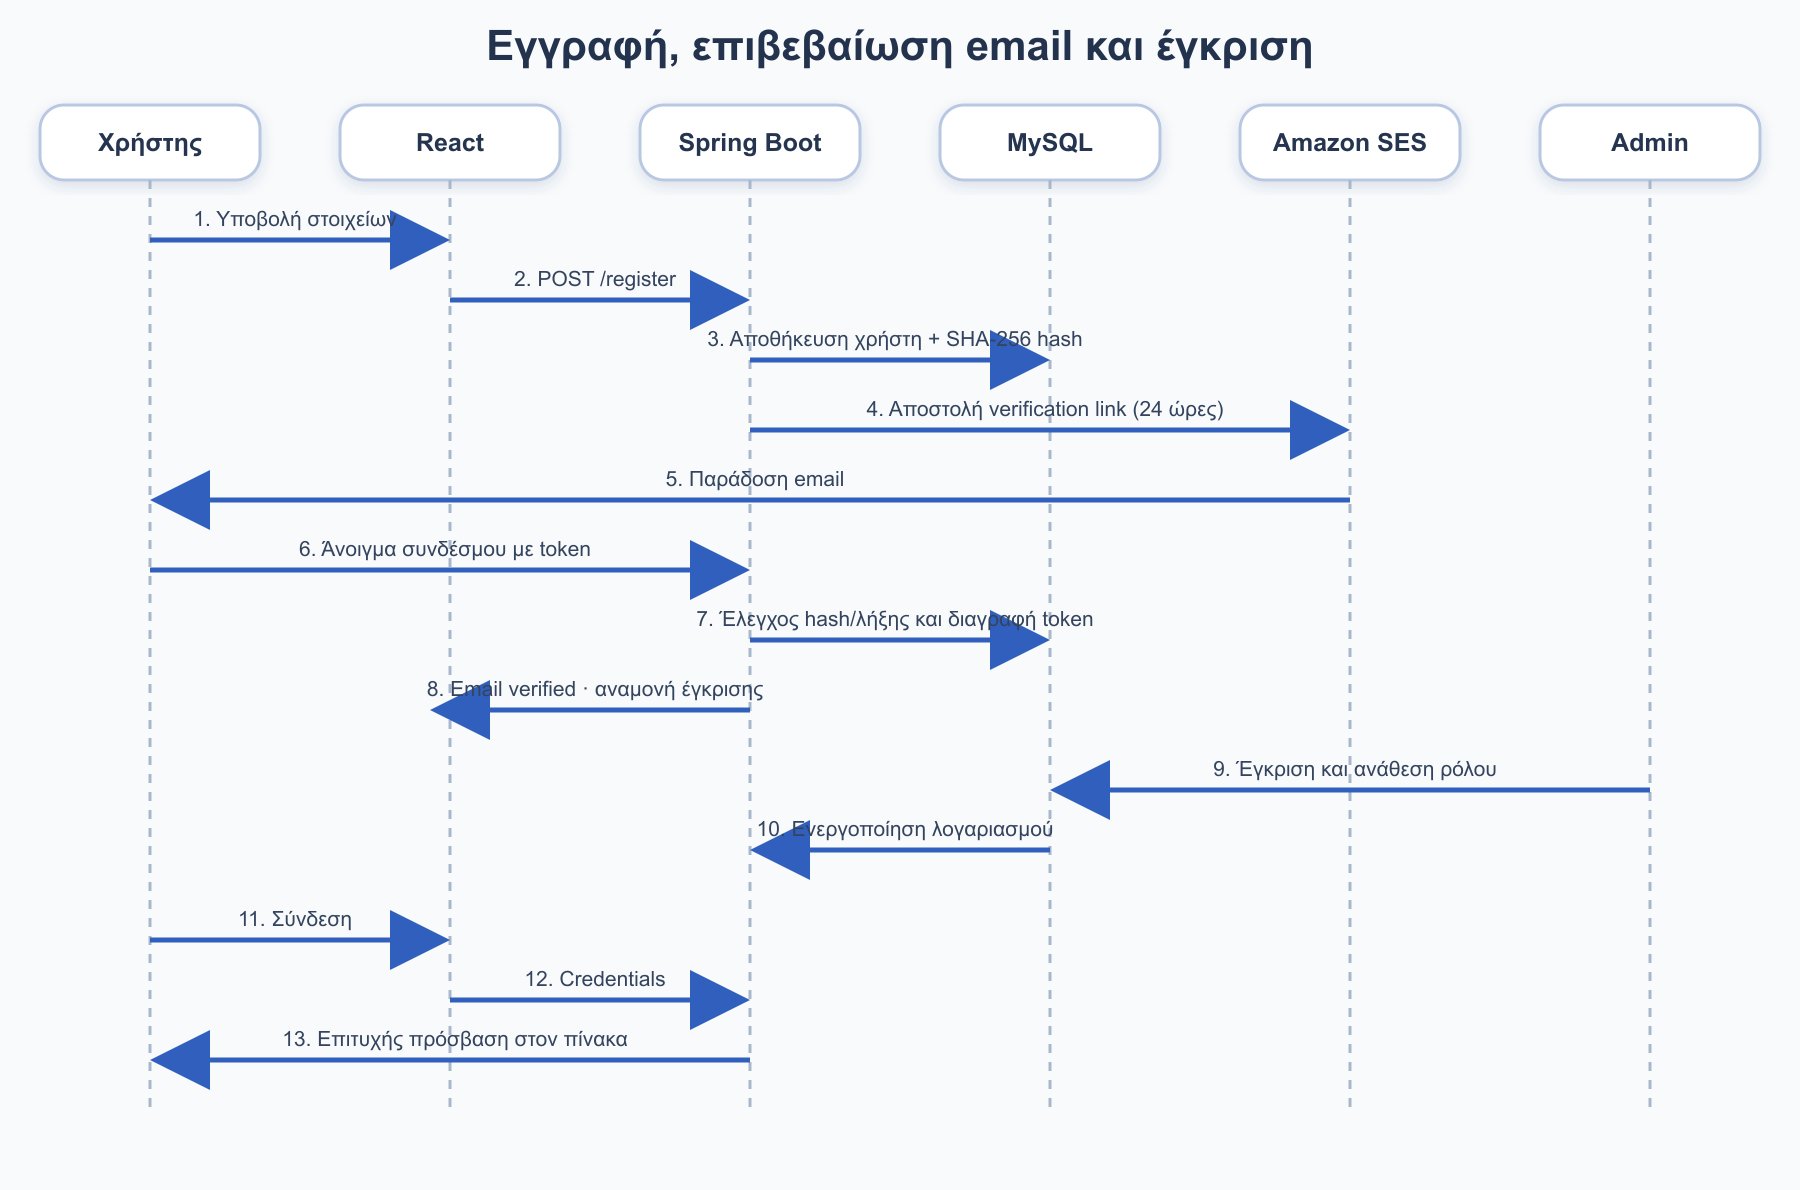
\includegraphics[width=\textwidth]{figures/application/registration-verification-sequence.png}
\caption{Ακολουθία εγγραφής, επιβεβαίωσης email και έγκρισης λογαριασμού.
Το token αποστέλλεται στον χρήστη, ενώ στη βάση αποθηκεύεται μόνο το hash
του. Η δυνατότητα σύνδεσης παρέχεται μετά την ανεξάρτητη έγκριση του
administrator.}
\label{fig:registration-verification-sequence}
\end{figure}

\section{Εγκατάσταση της εφαρμογής στην AWS}
Δημιουργήθηκε EC2 instance με Amazon Linux~2023, instance type
\texttt{t3.small}, EBS volume \texttt{gp3} 30~GiB και RSA key pair σε μορφή
OpenSSH. Κατά τη δημιουργία αντιστοιχίστηκε το security group της εφαρμογής
και, μετά την εκκίνηση, το instance έφθασε σε κατάσταση \texttt{Running} και
ολοκλήρωσε επιτυχώς τους ελέγχους κατάστασης της AWS. Η διαχειριστική σύνδεση
ελέγχθηκε μέσω SSH, ενώ η πρόσβαση στη θύρα 22 περιορίστηκε στην τρέχουσα
δημόσια IPv4 διεύθυνση του διαχειριστή με prefix \texttt{/32}. Η διεύθυνση
αυτή μπορεί να ενημερώνεται όταν μεταβάλλεται η σύνδεση του τοπικού δικτύου,
χωρίς να ανοίγει το SSH στο σύνολο του Internet.

Η διαδικασία δημιουργίας καταγράφηκε ως ακολουθία επαναλήψιμων βημάτων:
επιλογή Region και λειτουργικού συστήματος, διαμόρφωση compute και storage,
δημιουργία key pair και security group, εκκίνηση του instance, εγκατάσταση
του Docker runtime και ανάπτυξη των τριών containers.

\begin{figure}[htbp]
\centering
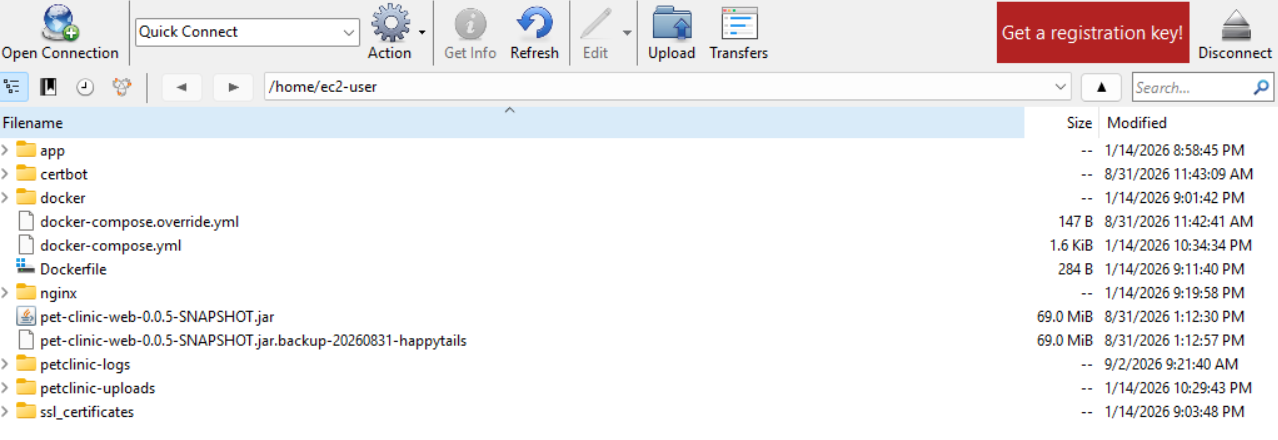
\includegraphics[width=0.95\textwidth]{figures/infrastructure/deployment-sftp-files.png}
\caption{Δομή των αρχείων deployment στο EC2 instance κατά την ασφαλή
διαχείριση μέσω SFTP. Διακρίνονται τα αρχεία Docker Compose, το application
JAR και οι κατάλογοι Nginx, πιστοποιητικών, logs και μεταφορτωμένων αρχείων.}
\label{fig:deployment-sftp-files}
\end{figure}

\begin{table}[htbp]
\caption{Έλεγχοι επαλήθευσης μετά τη δημιουργία της υποδομής και το deployment.}
\label{tab:deployment-verification}
\centering
\begin{tabularx}{\textwidth}{@{}p{4cm}p{3cm}X@{}}
\toprule
\textbf{Έλεγχος} & \textbf{Αναμενόμενο αποτέλεσμα} & \textbf{Καταγεγραμμένο αποτέλεσμα} \\
\midrule
EC2 status checks & 3/3 checks passed & Επιτυχής ολοκλήρωση και των τριών ελέγχων. \\
systemd failed units & Καμία αποτυχημένη μονάδα & Δεν εντοπίστηκαν failed units μετά την εκκίνηση. \\
Docker containers & Τρία containers σε λειτουργία & Spring Boot, MySQL και Nginx σε κατάσταση running. \\
MySQL health check & Healthy & Ο ενσωματωμένος health check ολοκληρώθηκε επιτυχώς. \\
Local HTTP request & HTTP 200 & Ο Nginx επέστρεψε επιτυχή απόκριση από το ίδιο το instance. \\
External DNS & Root και \texttt{www} στην Elastic IP & Και τα δύο ονόματα επιλύθηκαν στη \texttt{3.127.189.11}. \\
HTTP to HTTPS & HTTP 301 & Επιβεβαιώθηκε η μόνιμη ανακατεύθυνση. \\
HTTPS request & HTTP 200 και έγκυρο certificate & Επιβεβαιώθηκε εξωτερικά η ασφαλής πρόσβαση στην εφαρμογή. \\
\bottomrule
\end{tabularx}
\end{table}
\section{Παραμετροποίηση βάσης δεδομένων και μεταναστεύσεων}
Η MySQL~8.4 εκτελείται σε ανεξάρτητο container και δεν εκτίθεται ως δημόσια
υπηρεσία. Στο host η θύρα 3306 προσδένεται μόνο στη διεύθυνση
\texttt{127.0.0.1}, ενώ η εφαρμογή συνδέεται με το όνομα της υπηρεσίας
\texttt{petclinic-mysql} μέσω του εσωτερικού δικτύου Docker. Το όνομα της
βάσης και τα credentials παρέχονται από το αρχείο environment. Η MySQL
ρυθμίζεται με σύνολο χαρακτήρων \texttt{utf8mb4} και collation
\texttt{utf8mb4\_unicode\_ci}, ώστε να αποθηκεύονται χωρίς απώλεια ελληνικά
ονόματα και κείμενα.

Η διατήρηση των δεδομένων εξασφαλίζεται από το named volume
\texttt{mysql-data}, το οποίο προσαρτάται στο \texttt{/var/lib/mysql}. Έτσι,
η αντικατάσταση ή αναδημιουργία του container δεν συνεπάγεται διαγραφή των
δεδομένων. Ο ενσωματωμένος έλεγχος \texttt{mysqladmin ping} πρέπει να
ολοκληρωθεί επιτυχώς πριν ξεκινήσει η υπηρεσία Spring Boot. Η εξάρτηση αυτή
περιορίζει τις αποτυχημένες εκκινήσεις που θα προκαλούσε μία βάση η οποία
βρίσκεται ακόμη στο στάδιο αρχικοποίησης.

Η εξέλιξη του σχήματος καταγράφεται με Liquibase. Το κεντρικό αρχείο
\path{db.changelog-master.yaml} συμπεριλαμβάνει με σταθερή σειρά τα
changesets για τις σχέσεις ραντεβού, ιδιοκτήτη και κατοικίδιου, την
επιβεβαίωση email και τα tokens επαναφοράς κωδικού. Κατά την εκκίνηση, το
Liquibase συγκρίνει τα changesets με τους πίνακες
\path{DATABASECHANGELOG} και \path{DATABASECHANGELOGLOCK} και εφαρμόζει
μόνο όσα δεν έχουν ήδη εκτελεστεί. Με αυτόν τον τρόπο η ίδια έκδοση της
εφαρμογής μπορεί να αναπτυχθεί σε κενή ή υφιστάμενη βάση χωρίς χειροκίνητες
εντολές SQL.

Η ρύθμιση Hibernate DDL μπορεί να μεταβάλλεται μέσω environment variable.
Για αυστηρό production έλεγχο είναι προτιμότερη η τιμή
\texttt{validate}, ώστε το Hibernate να επιβεβαιώνει το σχήμα χωρίς να το
τροποποιεί και οι αλλαγές να παραμένουν αποκλειστική ευθύνη του Liquibase.
Η επαλήθευση πραγματοποιήθηκε με ελεγχόμενη επανεκκίνηση μόνο του Spring
container. Το Liquibase ανέγνωσε τον πίνακα \texttt{DATABASECHANGELOG},
ανέφερε τέσσερα changesets ως ήδη εκτελεσμένα, μηδενικές νέες εκτελέσεις και
επιτυχή αποδέσμευση του changelog lock. Συμπληρωματικό read-only ερώτημα στον
πίνακα επιβεβαίωσε τη σειρά και την κατάσταση \texttt{EXECUTED} και για τις
τέσσερις εγγραφές. Μετά την ολοκλήρωση, το container παρέμεινε σε κατάσταση
\texttt{Up} και η δημόσια διαδρομή επέστρεψε HTTPS~200. Η
Εικόνα~\ref{fig:liquibase-migrations} παρουσιάζει το σχετικό output χωρίς
credentials ή δεδομένα της εφαρμογής.

\begin{figure}[htbp]
\centering
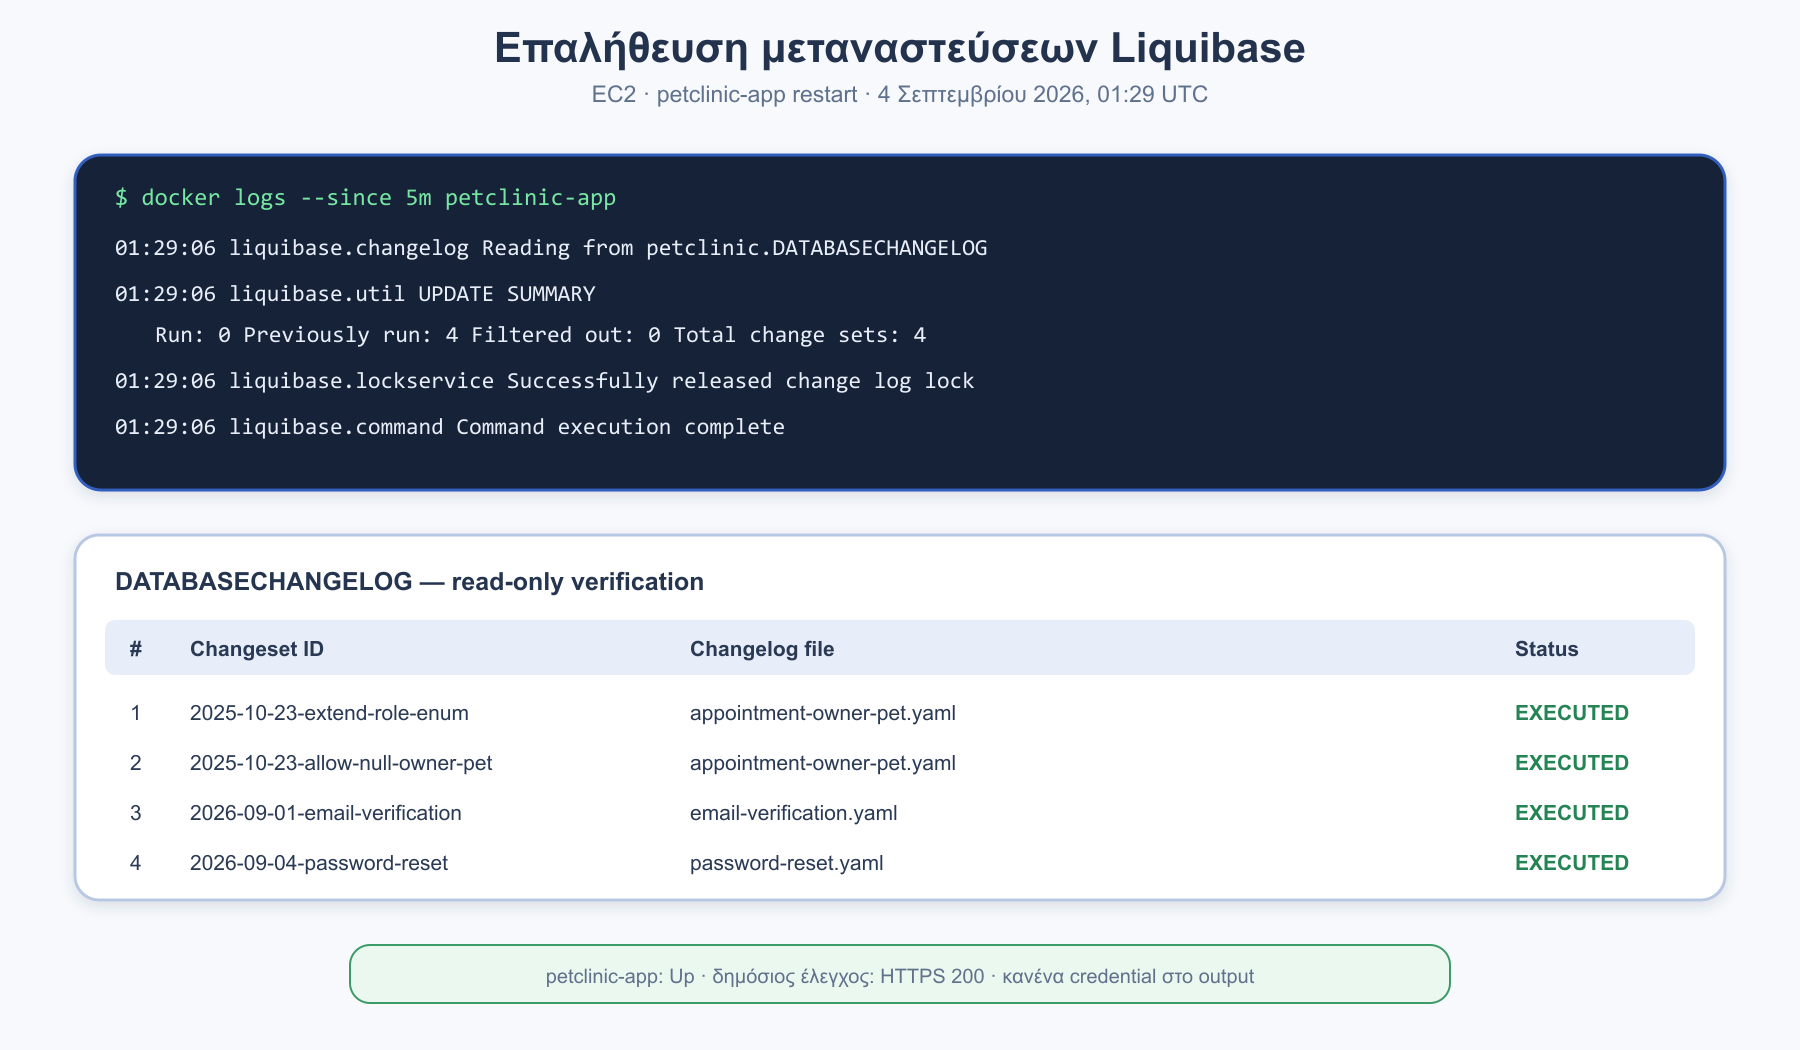
\includegraphics[width=\textwidth]{figures/infrastructure/liquibase-migrations.png}
\caption{Επαλήθευση Liquibase μετά από επανεκκίνηση του Spring container. Τα
startup logs δείχνουν ότι το schema ήταν ενημερωμένο, ενώ το read-only
ερώτημα στον πίνακα \texttt{DATABASECHANGELOG} επιβεβαιώνει τα τέσσερα
changesets που έχουν εφαρμοστεί.}
\label{fig:liquibase-migrations}
\end{figure}

\section{Διαχείριση στατικών και μεταφορτωμένων αρχείων}
Η παραγωγική έκδοση του React frontend δημιουργείται πριν από την παραγωγή
του Spring Boot JAR και διανέμεται μαζί με την εφαρμογή. Ο Nginx αποτελεί το
δημόσιο σημείο εισόδου και προωθεί τα αιτήματα στο backend, ενώ η ρύθμιση SPA
δρομολογεί τις client-side διαδρομές στο αρχικό έγγραφο της React. Με αυτόν
τον τρόπο δεν απαιτείται ξεχωριστός δημόσιος file server για τα στατικά
αρχεία της διεπαφής.

Τα έγγραφα του ιατρικού ιστορικού αποθηκεύονται από το
\path{DocumentStorageService} κάτω από τον κατάλογο
\path{/app/uploads/pet-documents}. Για κάθε κατοικίδιο δημιουργείται
ξεχωριστός υποκατάλογος και το φυσικό όνομα του αρχείου παράγεται από
timestamp και UUID. Η βάση δεδομένων διατηρεί τα μεταδεδομένα που χρειάζεται
η εφαρμογή, όπως το αρχικό όνομα, το content type, το μέγεθος και τη σχετική
διαδρομή. Ο διαχωρισμός αυτός επιτρέπει στη διεπαφή να εμφανίζει κατανοητό
όνομα χωρίς να χρησιμοποιεί το όνομα του χρήστη ως φυσικό όνομα αποθήκευσης.

Τόσο το Spring multipart configuration όσο και η υπηρεσία αποθήκευσης
επιβάλλουν μέγιστο μέγεθος 10~MB ανά αρχείο. Πριν από την ανάγνωση μιας
διαδρομής πραγματοποιούνται κανονικοποίηση και έλεγχος ότι το τελικό path
παραμένει εντός του ριζικού καταλόγου αποθήκευσης. Οι σχετικές unit tests
καλύπτουν σχετικές διαδρομές, διαχωριστικά Windows, αποθηκευμένες διαδρομές
με prefix, ανύπαρκτα αρχεία και απόρριψη αρχείου μεγαλύτερου από το όριο.

Ο κατάλογος \texttt{/app/uploads} προσαρτάται στο named volume
\texttt{petclinic-uploads}, ώστε τα έγγραφα να παραμένουν διαθέσιμα όταν
ανακατασκευάζεται μόνο το Spring container. Για τη λειτουργική επαλήθευση
μεταφορτώθηκε ένα τυχαίο PDF
έγγραφο, χωρίς συσχέτιση με πραγματικό ιατρικό περιστατικό. Η εφαρμογή το
κατέγραψε ως \texttt{application/pdf}, μεγέθους περίπου 1,1~MB, και το
εμφάνισε στη σχετική καρτέλα, όπως φαίνεται στην
Εικόνα~\ref{fig:uploaded-document-record}. Το πλήκτρο \enquote{Προβολή}
ανακτά επιτυχώς το αποθηκευμένο αρχείο και εμφανίζει το PDF στον browser,
επιβεβαιώνοντας και τη διαδρομή ανάγνωσης του συνημμένου. Το περιεχόμενο του
τυχαίου παραστατικού δεν συμπεριλαμβάνεται στην τεκμηρίωση, καθώς δεν αποτελεί
ιατρικό δεδομένο ούτε απαιτείται για την απόδειξη της λειτουργίας.

\begin{figure}[htbp]
\centering
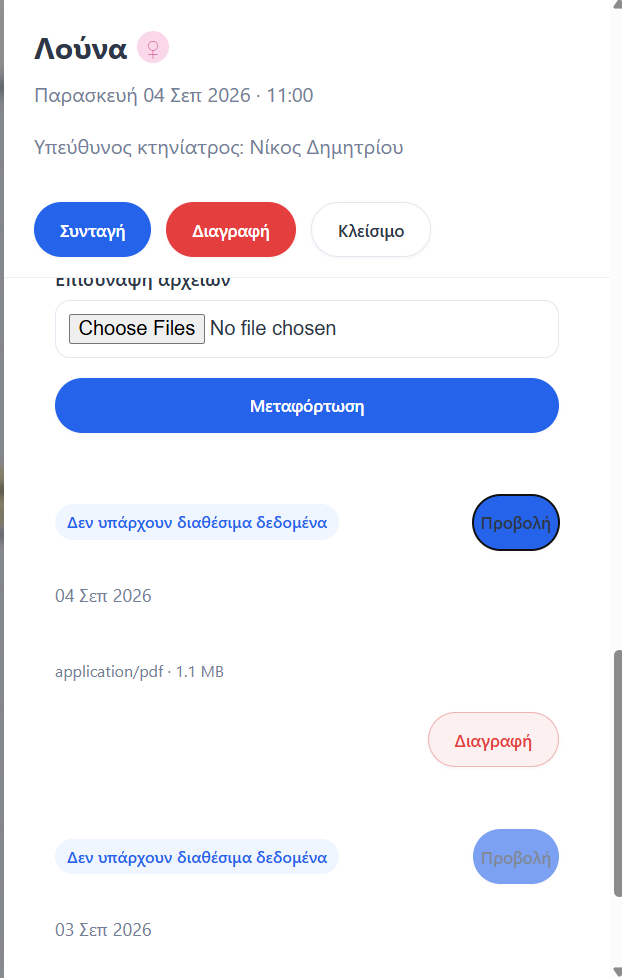
\includegraphics[width=0.46\textwidth]{figures/application/uploaded-document-record.png}
\caption{Επιτυχής αποθήκευση δοκιμαστικού PDF ως συνημμένου σε εγγραφή της
εφαρμογής. Διακρίνονται ο τύπος, το μέγεθος και το ενεργό πλήκτρο
\enquote{Προβολή}, μέσω του οποίου επαληθεύτηκε η επιτυχής ανάκτηση και
εμφάνιση του PDF, χωρίς να δημοσιοποιείται το περιεχόμενό του.}
\label{fig:uploaded-document-record}
\end{figure}

Πριν από την επανεκκίνηση καταγράφηκαν η παραγόμενη διαδρομή, το ακριβές
μέγεθος των 1.191.697 bytes και το SHA-256 checksum του αρχείου. Μετά από
επανεκκίνηση αποκλειστικά του \texttt{petclinic-app}, η ίδια διαδρομή
παρέμεινε διαθέσιμη με αμετάβλητο μέγεθος και checksum, ενώ η δημόσια
διαδρομή της εφαρμογής επέστρεψε HTTPS~200. Το αποτέλεσμα επιβεβαιώνει ότι το
αρχείο βρίσκεται στο persistent volume και όχι στο προσωρινό writable layer
του container. Η συγκεντρωτική απεικόνιση της δοκιμής έχει προετοιμαστεί για
την αξιολόγηση αξιοπιστίας του Κεφαλαίου~6.

\section{Ρύθμιση DNS, HTTPS και αντίστροφου διακομιστή μεσολάβησης}
Ο Nginx προωθεί τα αιτήματα προς την υπηρεσία Spring Boot στη θύρα 8080 του
εσωτερικού δικτύου Docker και διατηρεί τις επικεφαλίδες
\texttt{X-Real-IP}, \texttt{X-Forwarded-For} και
\texttt{X-Forwarded-Proto}. Η δημόσια πρόσβαση γίνεται μέσω των εγγραφών
Route~53 και της σταθερής Elastic IP. Για την έκδοση του πιστοποιητικού
χρησιμοποιήθηκε η μέθοδος HTTP-01 του Let's Encrypt για τα δύο δημόσια
ονόματα. Ο Nginx ρυθμίστηκε για TLS~1.2 και TLS~1.3 και επιστρέφει ανακατεύθυνση
301 από HTTP προς HTTPS. Η ανανέωση εκτελείται καθημερινά από χρονοδιακόπτη
systemd, ο οποίος εκκινεί προσωρινό container Certbot και στη συνέχεια
επαναφορτώνει τη ρύθμιση του Nginx. Μετά τη ρύθμιση επαληθεύτηκαν η ορθότητα
του αρχείου Nginx, απόκριση HTTPS~200 και η κανονική προβολή της εφαρμογής.

\begin{figure}[htbp]
\centering
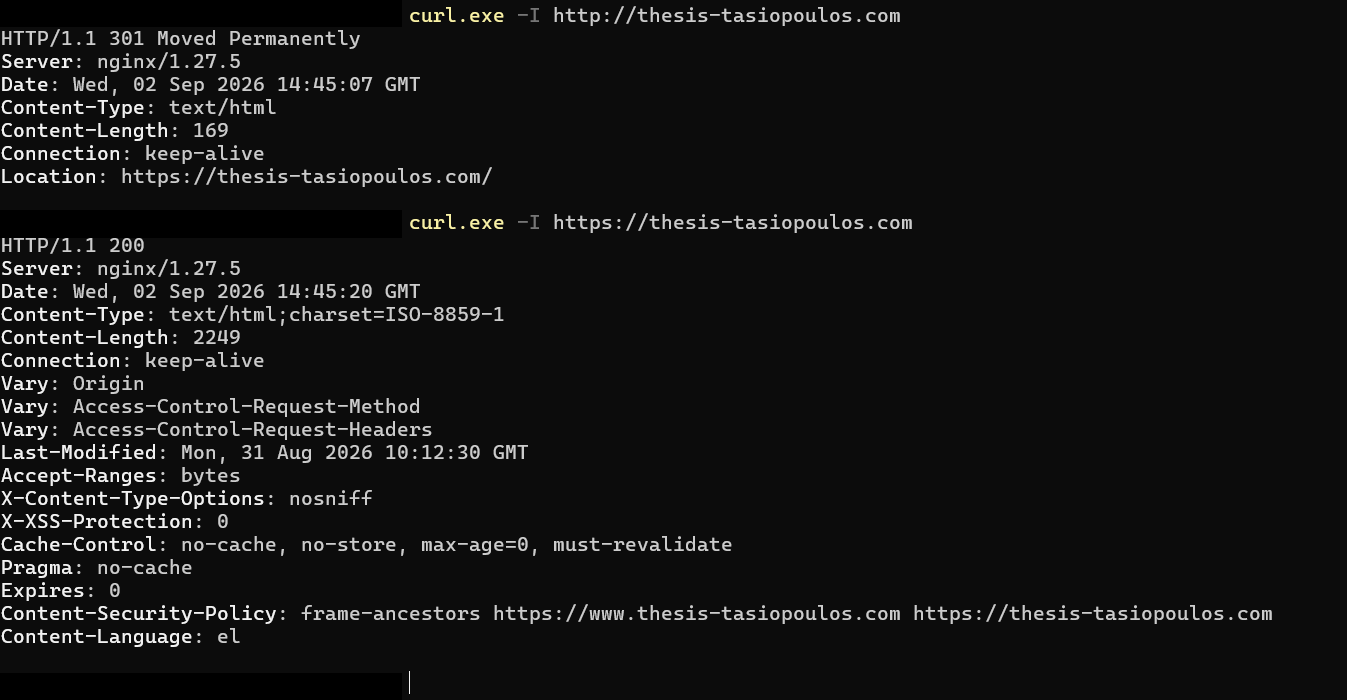
\includegraphics[width=0.96\textwidth]{figures/infrastructure/http-https-verification.png}
\caption{Εξωτερικός έλεγχος της δημόσιας πρόσβασης: το HTTP endpoint
επιστρέφει μόνιμη ανακατεύθυνση 301 προς HTTPS, ενώ το HTTPS endpoint
επιστρέφει επιτυχή απόκριση 200. Η τοπική διαδρομή χρήστη έχει αποκρυφθεί.}
\label{fig:http-https-verification}
\end{figure}
\section{Παρακολούθηση λειτουργίας και αντίγραφα ασφαλείας}
Η αρχική επαλήθευση περιέλαβε τους ελέγχους κατάστασης EC2, την κατάσταση
υγείας του container της MySQL, την κατάσταση των τριών containers και
αίτημα HTTP προς τον Nginx. Η εφαρμογή επέστρεψε κωδικό 200 και η αρχική
ελληνική σελίδα προβλήθηκε επιτυχώς σε εξωτερικό πρόγραμμα περιήγησης. Η
τελική αξιολόγηση συμπληρώθηκε με βασικά EC2 metrics και status checks από
το CloudWatch, έλεγχο των πραγματικών παραγόντων κόστους και καταγραφή της
συμπεριφοράς της εγκατάστασης κατά την επανεκκίνηση. Τα αντίστοιχα
αποτελέσματα, οι χρονικές περίοδοι μέτρησης και οι περιορισμοί παρουσιάζονται
αναλυτικά στο Κεφάλαιο~6. Η δοκιμή επιβεβαίωσε τη διατήρηση δεδομένων στο
υπάρχον instance, όχι όμως πλήρες restore από snapshot σε νέο περιβάλλον.
\section{Διαδικασία ενημέρωσης και επανεκκίνησης}
Η ενημέρωση της εφαρμογής περιλαμβάνει παραγωγή νέου JAR, μεταφορά του στο
instance, rebuild του Spring container και ελέγχους λειτουργίας, χωρίς να
απαιτείται αναδημιουργία της MySQL ή του Nginx. Η διαδικασία ενημέρωσης έχει
ήδη εφαρμοστεί σε αλλαγές της δημόσιας διεπαφής. Ο ελεγχόμενος reboot του
instance εκτελέστηκε ως χωριστό πείραμα. Καταγράφηκε ο χρόνος μέχρι την
επιστροφή της δημόσιας υπηρεσίας και επιβεβαιώθηκαν η αυτόματη εκκίνηση του
Docker, η προσάρτηση των persistent volumes και η κατάσταση των containers.
Το endpoint επανήλθε σε 40,79~s χωρίς απώλεια των ελεγχόμενων δεδομένων, όπως
τεκμηριώνεται στην Ενότητα~6.6.

\begin{figure}[htbp]
\centering
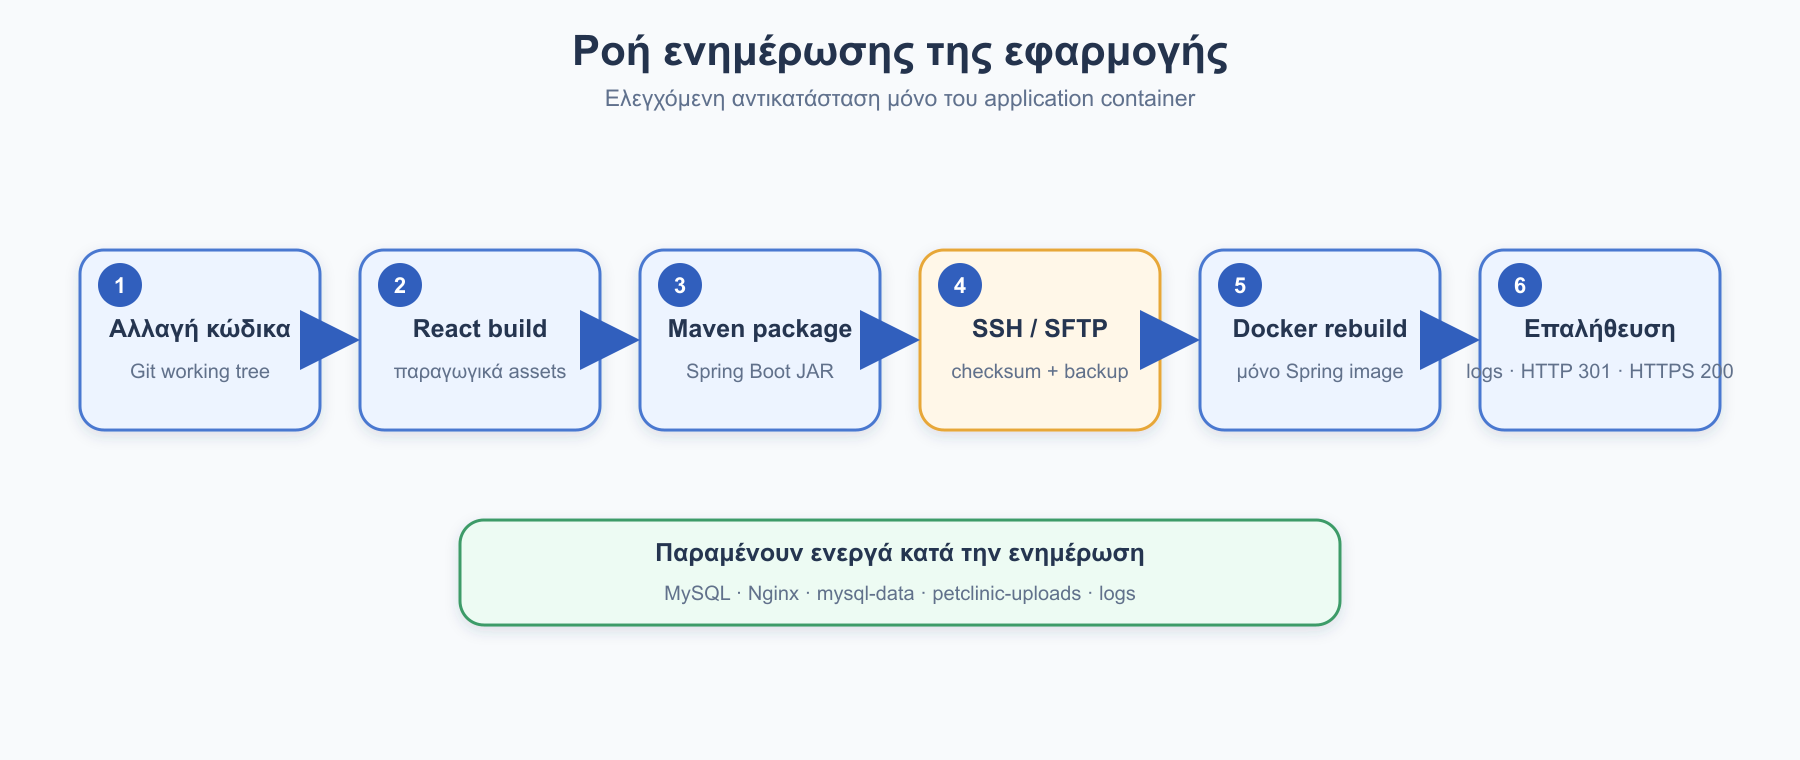
\includegraphics[width=\textwidth]{figures/infrastructure/deployment-pipeline.png}
\caption{Ροή ενημέρωσης και επαλήθευσης του application deployment. Κατά
την ανανέωση ανακατασκευάζεται μόνο το Spring image, ενώ η MySQL, ο Nginx και
τα persistent volumes παραμένουν ενεργά.}
\label{fig:deployment-pipeline}
\end{figure}
